\chapter{Expériences : analyse provisoire et liste}
\graphicspath{{04-Analyse/}}

Cette section présente les différentes expériences réalisées afin de mieux comprendre l'architecture CxSOM. C'est une section provisoire, elle permet de mettre en relation les expériences afin d'ensuite tirer des conclusions claires a propos de l'architetecture CxSOM.
En utilisant les indicateurs et tracés présentés dans le chapitre précédent, nous détaillons dans cette partie les résltats obtenus et les pistes d'interprétation.

Les jeux de données présentés aux cartes de l'architecture sont des nuages de points en deux ou trois dimensions, tirés selon une distribution.
Les données d'entrée à l'architecture de carte seront notées $X$,$Y$,$Z$, sauf mention contraire. Ces trois valeurs sont scalaires, sont les coordonnées d'un point du nuage de point, et correspondent chacune à l'entrée d'une des cartes de l'architecture.

Dans cette version, les notations ne sont pas encore homogènes: l'autrice s'en excuse d'avance. Notez donc que : 
les modalités $X\m{i}$ sont ici notées $I^i$. L'entrée $I^i$ est toujours assignée à la carte $M^i$. Lorsqu'on utilise la variable $M^i$, il s'agit de la position du BMU $\bmu\m{i}$.

\section{Entrées sur un cercle}

Une architecture de deux cartes, connectées mutuellement, est l'exemple le plus simple d'architecture CxSOM. Son étude permet de dégager des comportements facilement représentables d'un point de vue graphique et ayant peu de liberté possible. 


\subsection{Cercle 2 dimensions}
Prenons en entrée $(X,Y)$ situé sur n cercle de centre 0.5 et de rayon 0.5, tel que $X,Y \in [0,1]$. 
Les entrées de chacune des cartes sont donc dépendantes. Nous regarderons la distribution des valeurs selon les BMU de chaque carte.

\begin{figure}[h!]
\begin{minipage}{0.33\textwidth}
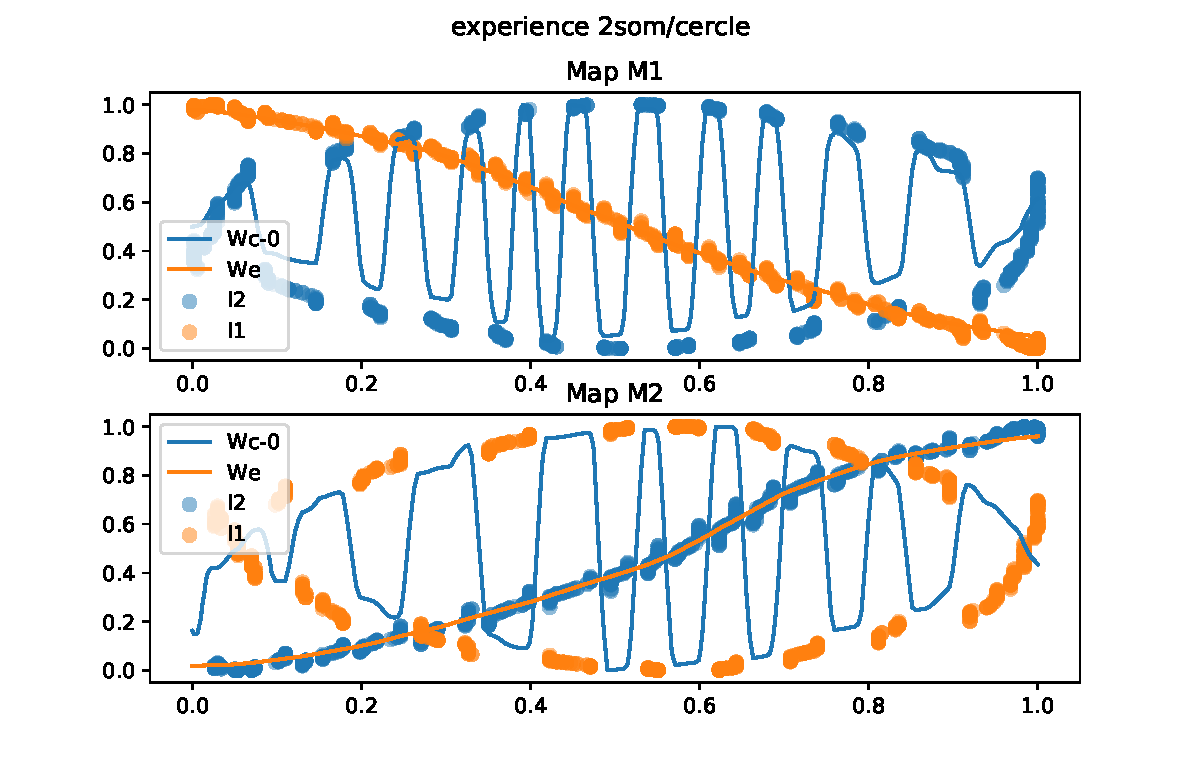
\includegraphics[width=\textwidth]{2som_cercle_w.pdf}
\end{minipage}
\begin{minipage}{0.33\textwidth}
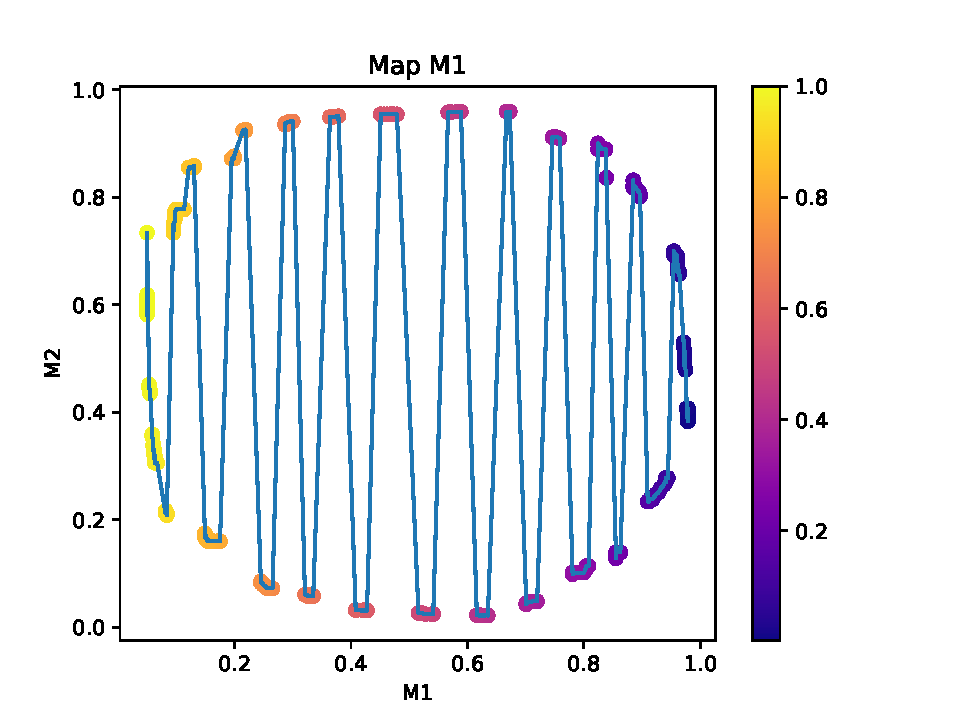
\includegraphics[width=\textwidth]{2som_cercle_d.pdf}
\end{minipage}
\begin{minipage}{0.33\textwidth}
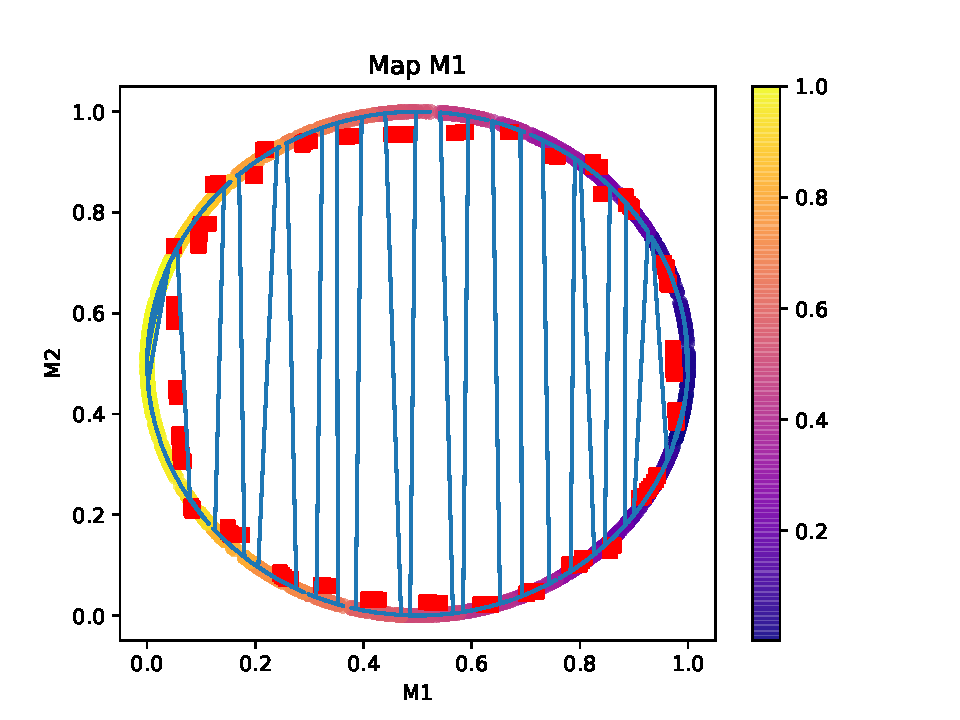
\includegraphics[width=\textwidth]{2som_cercle_din.pdf}
\end{minipage}
\label{fig:2som_square}
\caption{Tracé des poids de M1 et M2, dépliement des poids de M1 dans l'espace 2D et dépliement des entrées}
\end{figure}

\subsection{Cercle trois dimensions}

Les entrées sont $(X,Y,Z)$, trois cartes connectées mutuellement. Les entrées sont dépendantes de telle sorte à ce que connaitre l'une d'entre elle laisse 50\% d'erreur sur les deux autre, mais deux d'entre elle permettent de déterminer totalement la troisième. 

En figure~\ref{fig:3som_cercle}
\begin{figure}[h!]
\begin{minipage}{0.33\textwidth}
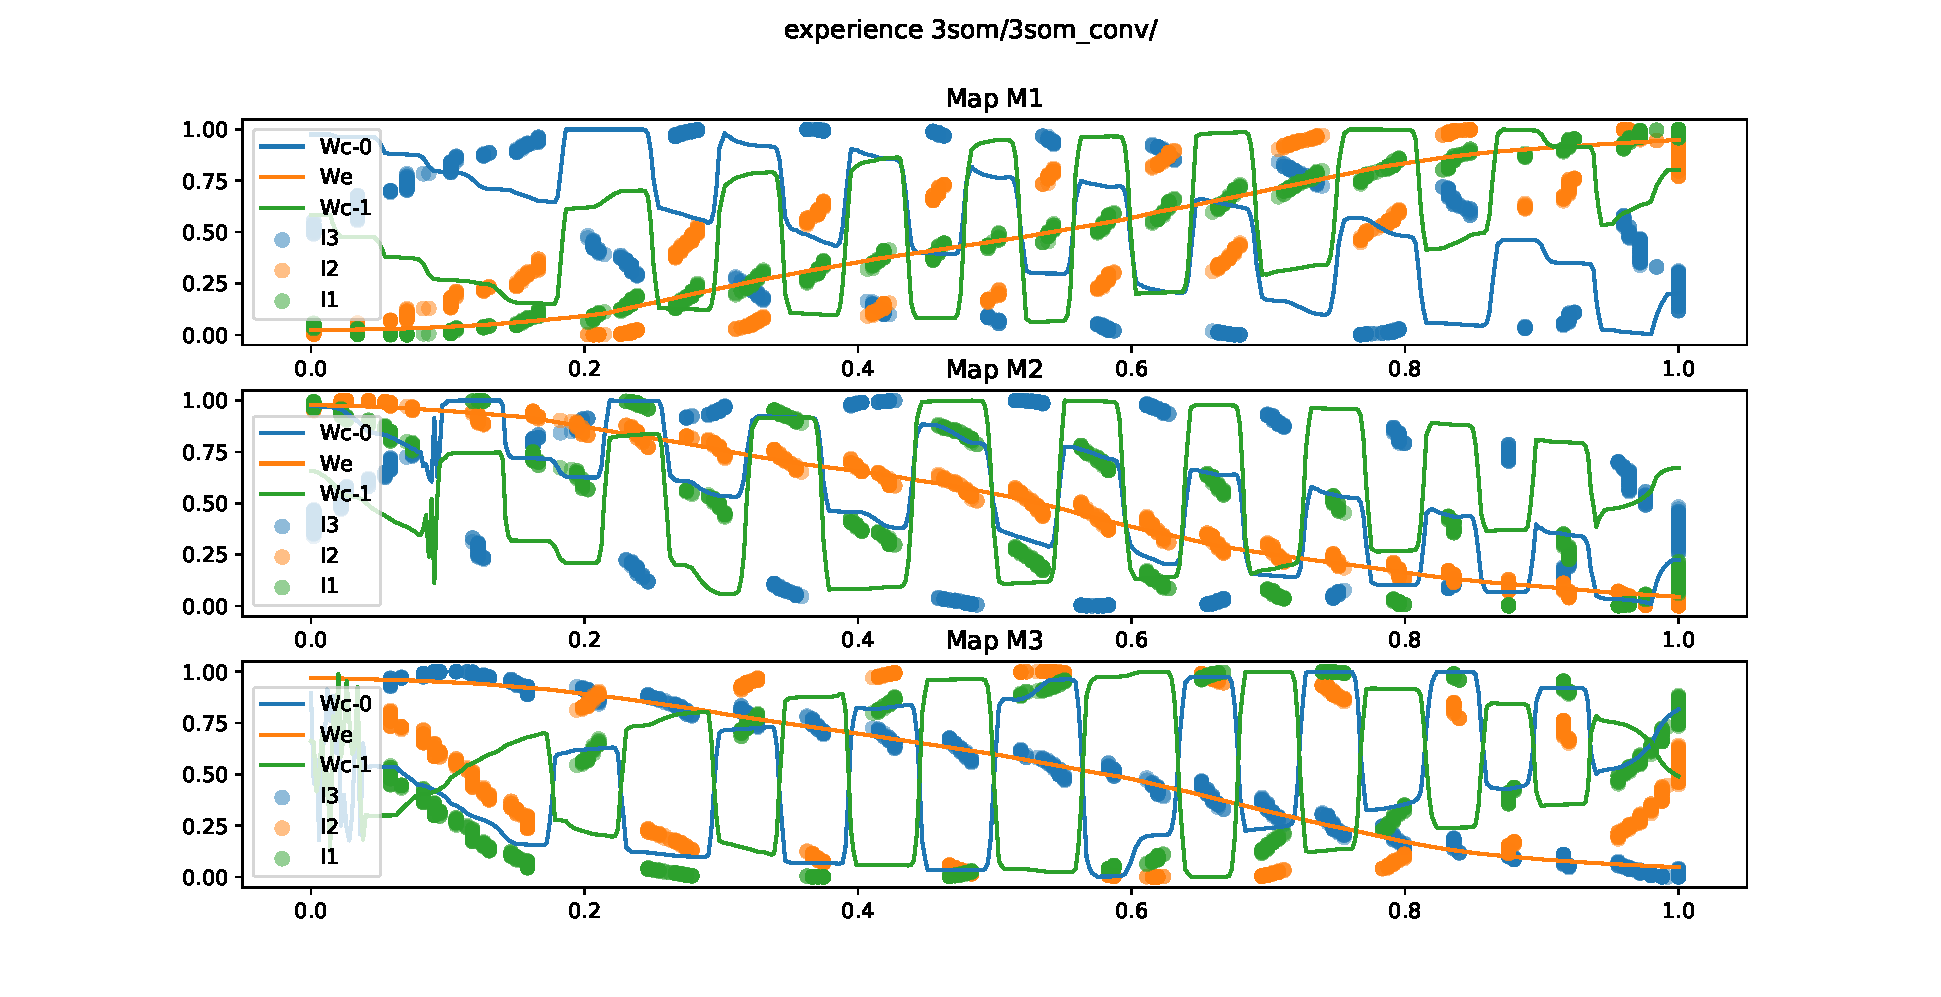
\includegraphics[width=\textwidth]{3som_cercle_w}
\end{minipage}
\begin{minipage}{0.33\textwidth}
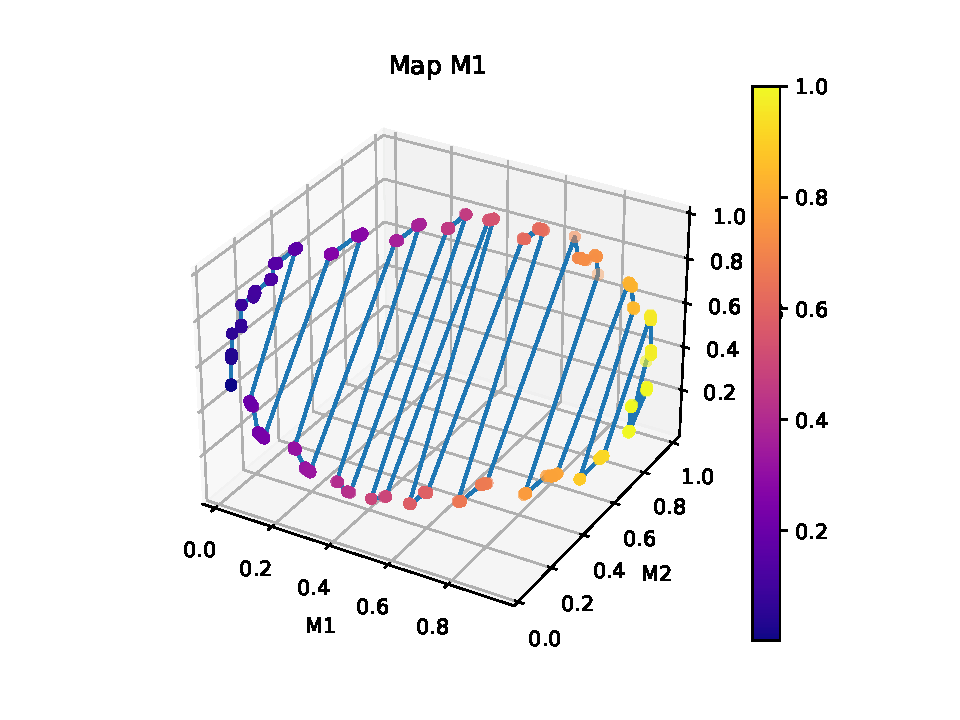
\includegraphics[width=\textwidth]{3som_cercle_dw1}
\end{minipage}
\begin{minipage}{0.33\textwidth}
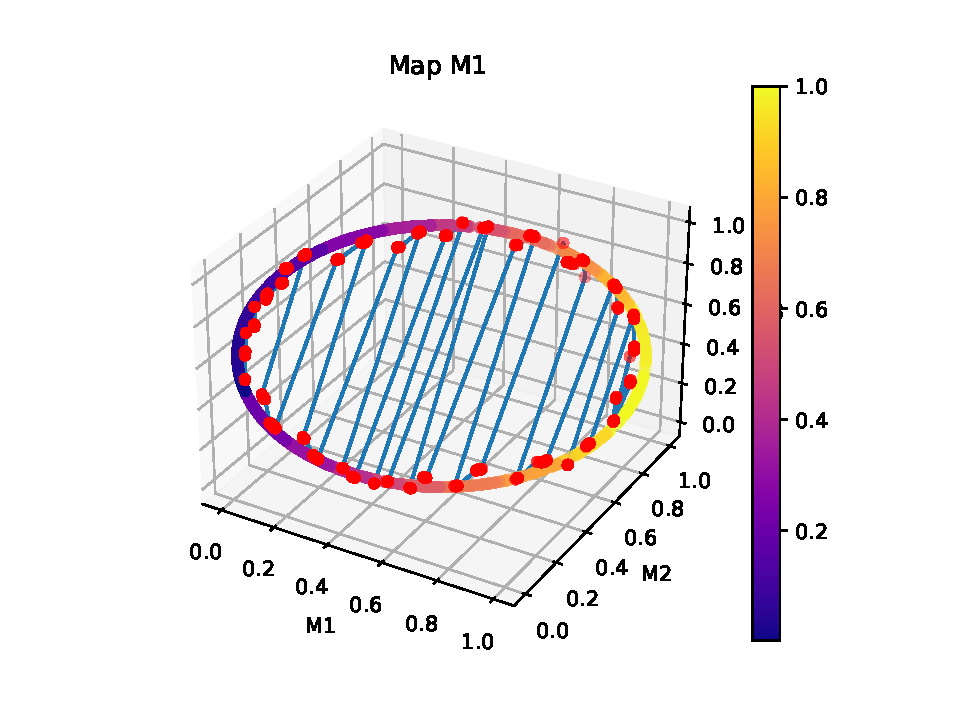
\includegraphics[width=\textwidth]{3som_cercle_din1}
\end{minipage}
\end{figure}
\begin{figure}
\centering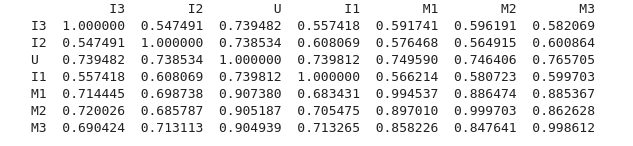
\includegraphics[width=0.8\textwidth]{3som_cercle_im}
\caption{Valeurs de $UC$ entre les différents éléments des cartes pour des entrées sur un cercle. Pour un élément $i,j$ du tableau est indiqué $UC(i|j)$ (Mi correspond à $\Pi\m{i}$. Le tableau sera mis au propre s'il est pertinent. Estimation par la méthode de Kraskov, voisinage de 7. Ce voisinage est arbitraire, il produit une variance plus grande mais biais moins important. Il faudrait refaire l'expé sur de multiple echantillons pour avoir une valeur sure. }
\label{fig:3som_cercle}
\end{figure}



\subsection{Entrées dans un anneau}

On peut, au lieu de considérer un cercle, ajouter du bruit à chaque dimension. Les entrées sont alors tirées dans un fin anneau ou tore. Dans ces conditions, le modèle peut toujours être considéré comme un cercle avec bruit. On peut donc prendre $U$ en une dimension :  
$$
 \begin{cases}
     X_t = r  \cos(U_t) + \epsilon_X\\
     Y_t = r \sin(U_t) + \epsilon_Y
    \end{cases}\,.
$$
Cenpendant, on peut aussi considérer que le modèle n'est plus réductible en une seule dimension cachée.
Il est donc intéressant de regarder comment les cartes considèrent le bruit : a-t-on toujours une quantification vectorielle du cercle, ou la carte se déplie t-elle autrement ? Autrement dit, une carte sépare t-elle le bruit de la forme des entrées ?

\begin{figure}
\centering
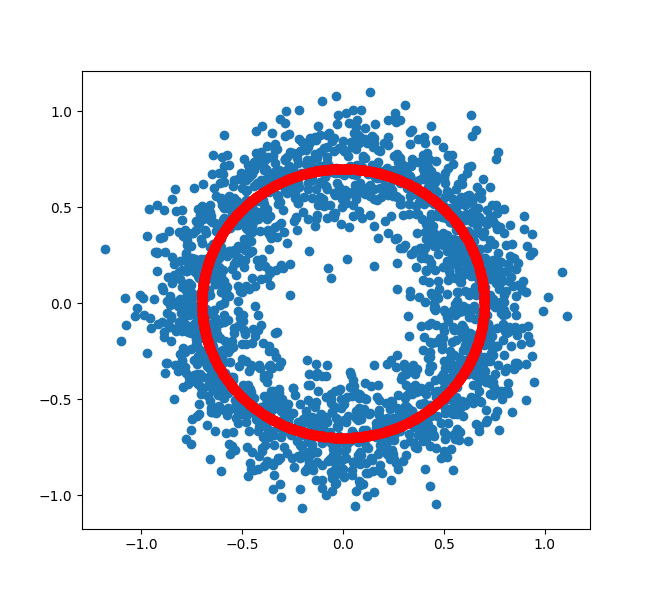
\includegraphics[width=0.4\textwidth]{inputs_anneau_cercle.png}
\caption{Entrées d'apprentissage en bleu, entrées test en rouge}
\label{fig:inputs_anneau_cercle}
\end{figure}

Pour le vérifier, on peut, à partir des poids appris sur des données bruitées, réaliser les tests sur des données non bruitée, donc un cercle, entrées présentées en figure~\ref{fig:inputs_anneau_cercle}.
Dans ce cas, la prédiction et la répartition est semblable au cas ou les cartes ont appris le cercle : la quantification est résistante au bruit, comme présenté en figure~\ref{fig:anneau_cercle}. On regardera donc par la suite le comportement des cartes sur des données non bruitées. 

\begin{figure}
\begin{minipage}{0.5\textwidth}
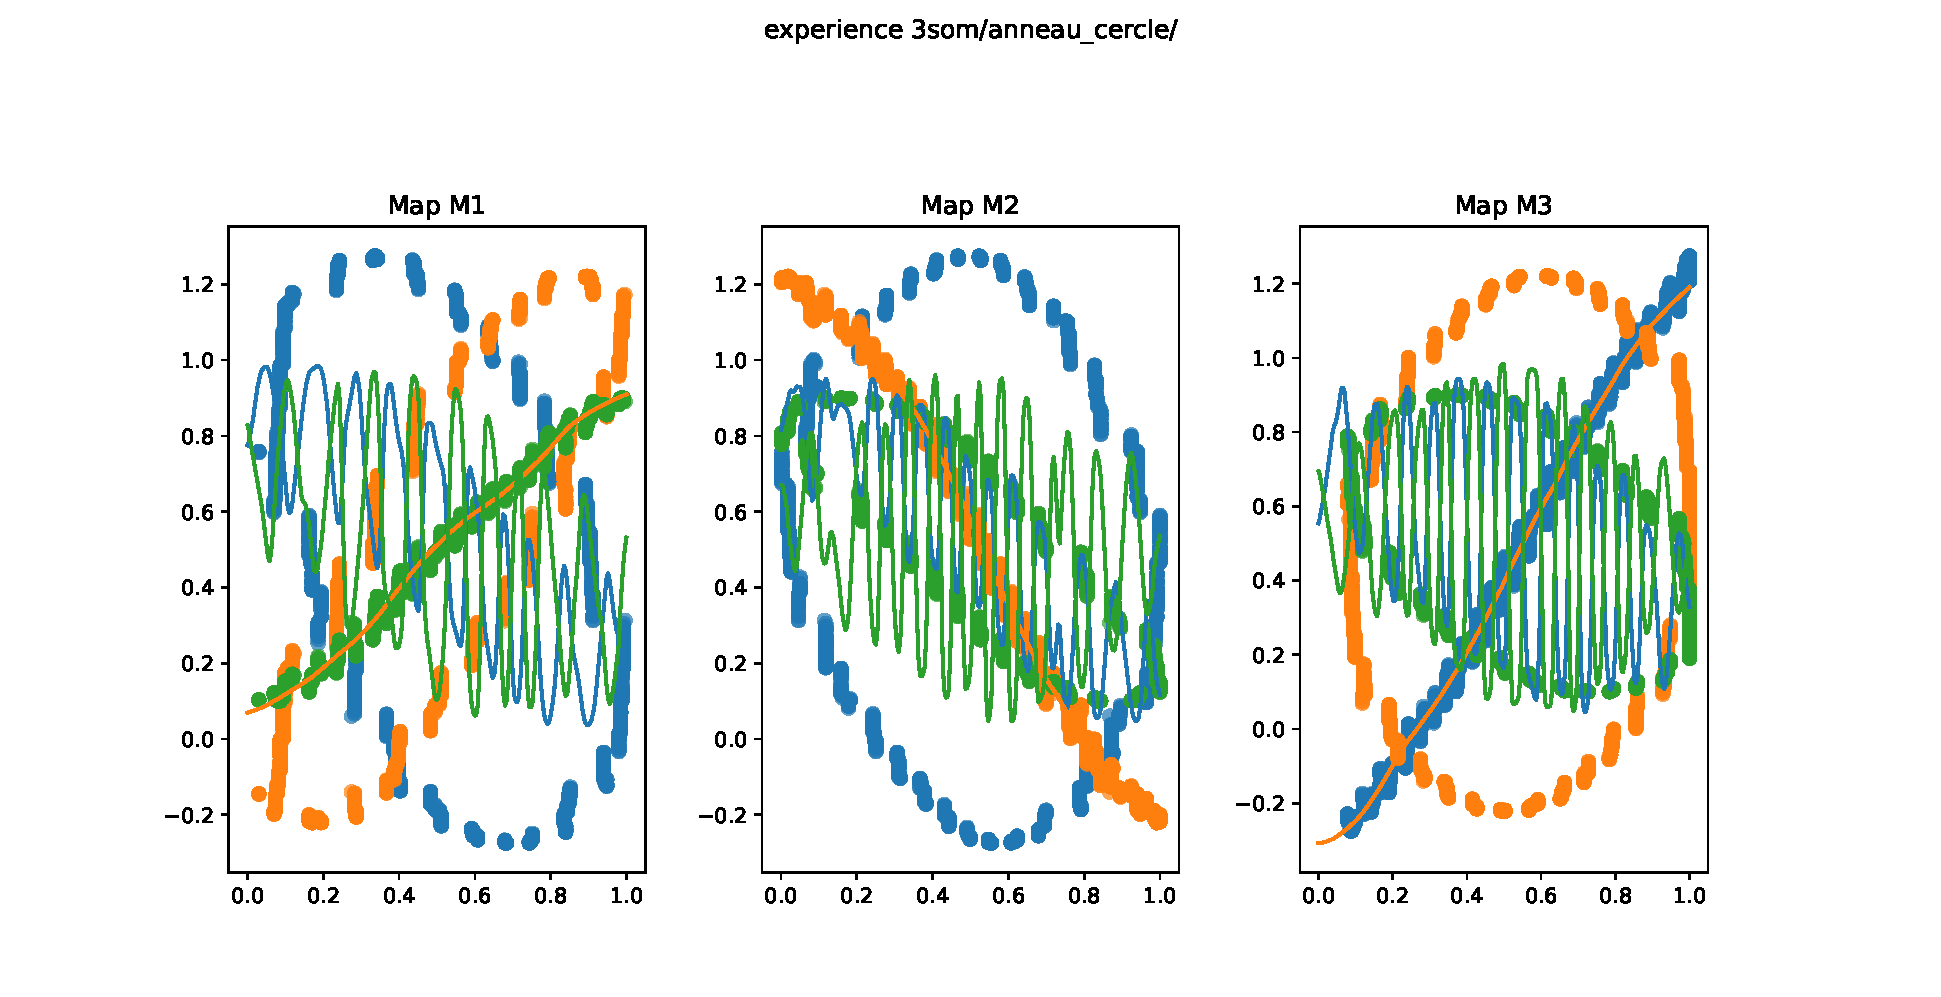
\includegraphics[width=\textwidth]{3som_anneau_cercle_w.pdf}
\end{minipage}
\begin{minipage}{0.5\textwidth}
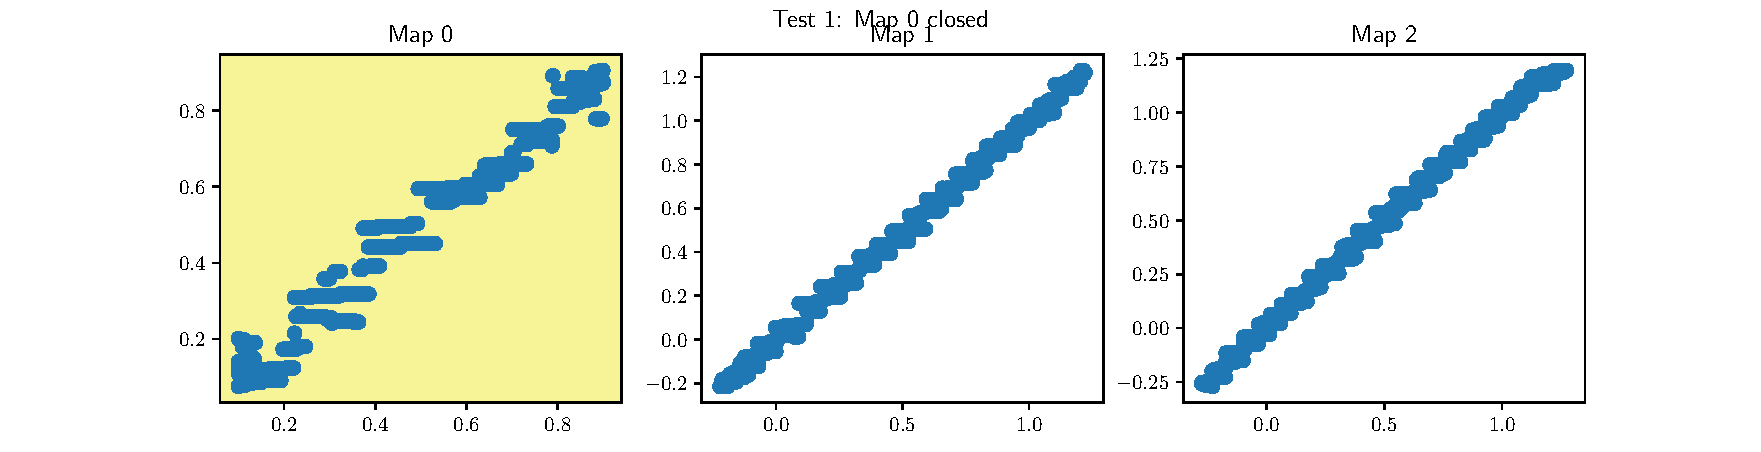
\includegraphics[width=\textwidth]{3som_anneau_cercle_pred.pdf}
\end{minipage}
\caption{L'apprentissage a été réalisé sur un cercle en 3D avec bruit, les tests sur le cercle. La répartition des entrées et poids et la prédiction est réalisée comme sur le cercle : la quantification vectorielle est résistante au bruit. }
\label{fig:anneau_cercle}
\end{figure}

\section{Entrées dans un carré}

\subsubsection{Expérience}
Prenons en entrée $(X,Y) \in [0,1]^2$, tirés selon une distribution uniforme. Les entrées de chacune des cartes sont donc indépendantes. Nous regarderons la distribution des valeurs selon les BMU de chaque carte. Cette distribution de valeurs dépendra donc uniquement de l'architecture, étant données que les entrées n'ont aucun lien entre elles. Cela nous permet de visualiser quels comportements sont uniquement issus du modèle.
 
\subsubsection{Résultats}

\begin{figure}[h!]
\begin{minipage}{0.33\textwidth}
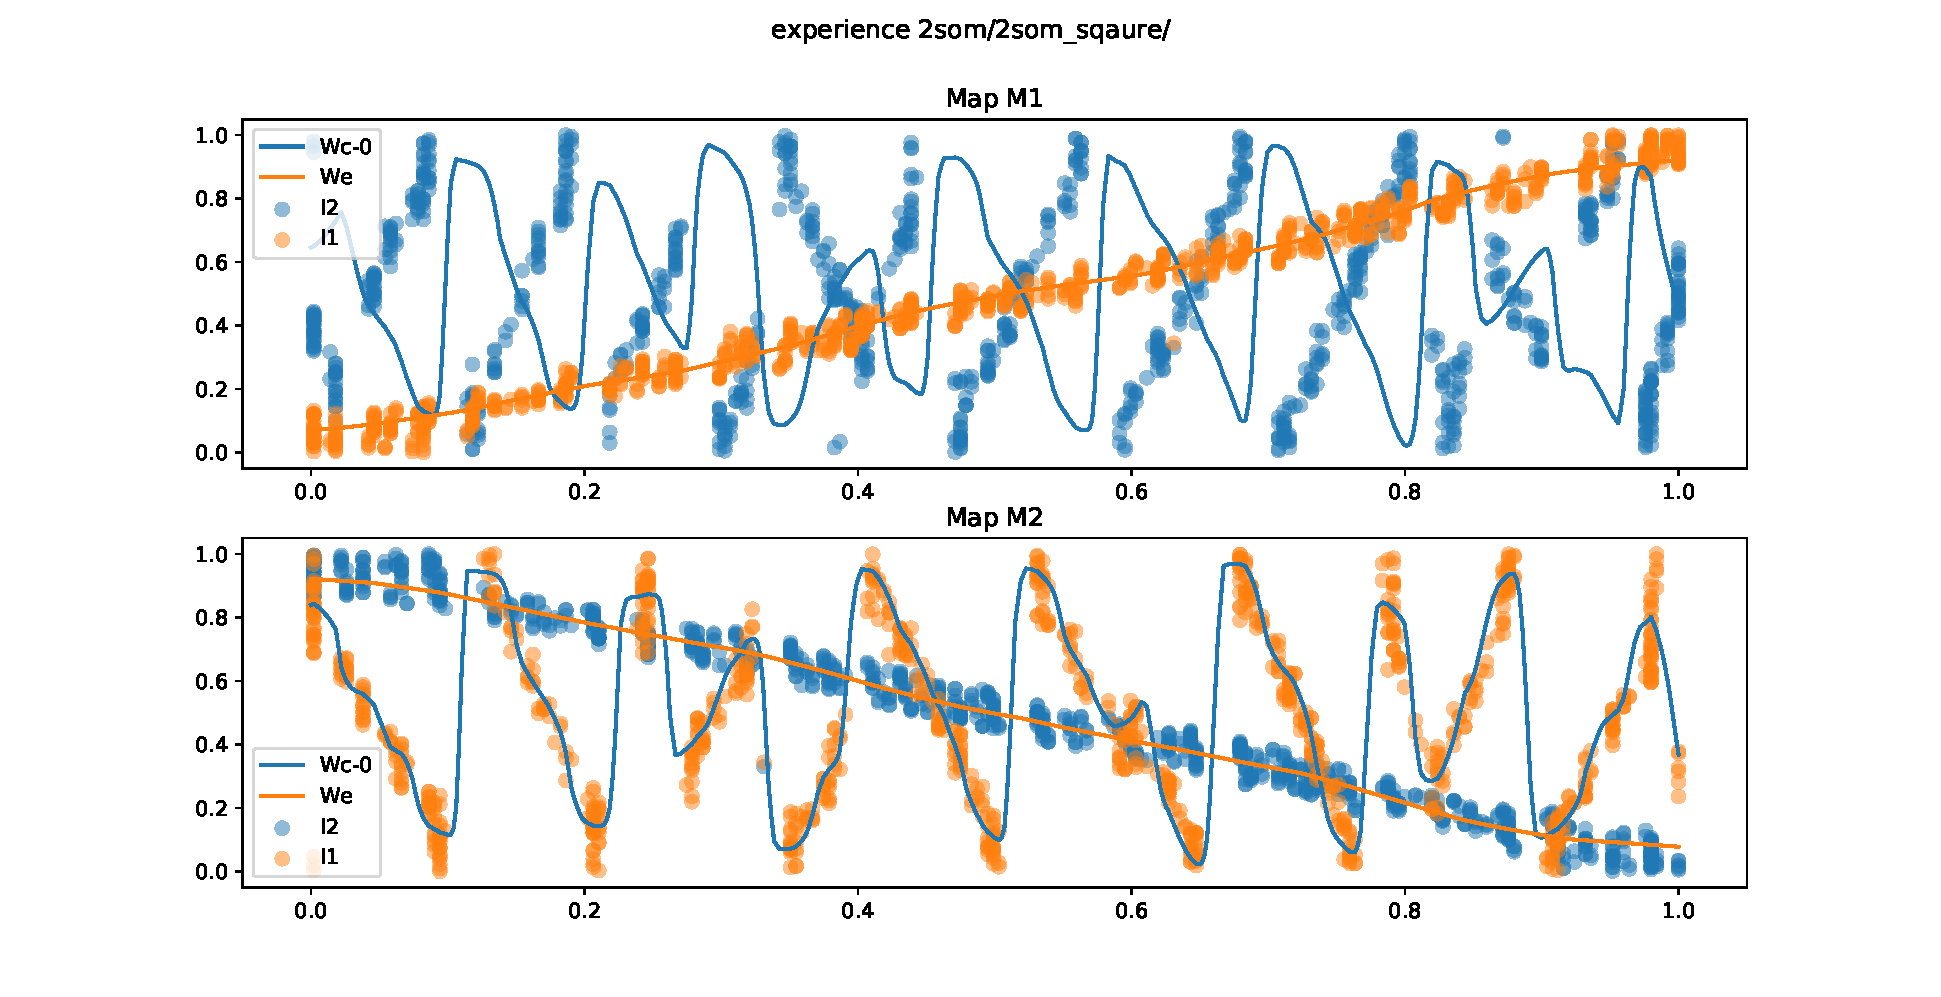
\includegraphics[width=\textwidth]{2som_square_w.pdf}
\end{minipage}
\begin{minipage}{0.33\textwidth}
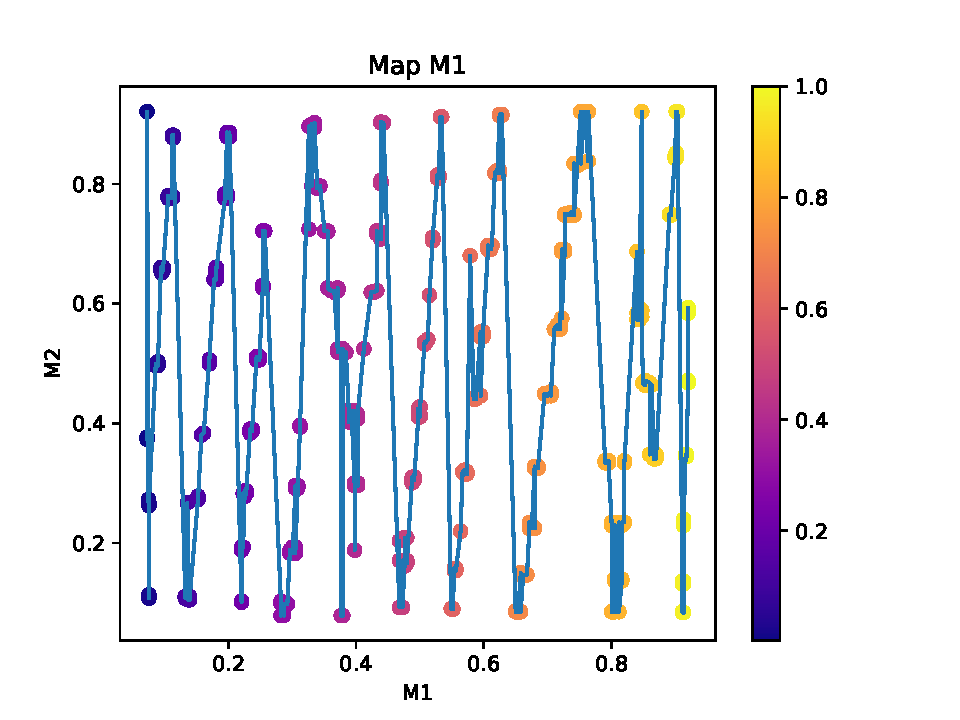
\includegraphics[width=\textwidth]{2som_square_d.pdf}
\end{minipage}
\begin{minipage}{0.33\textwidth}
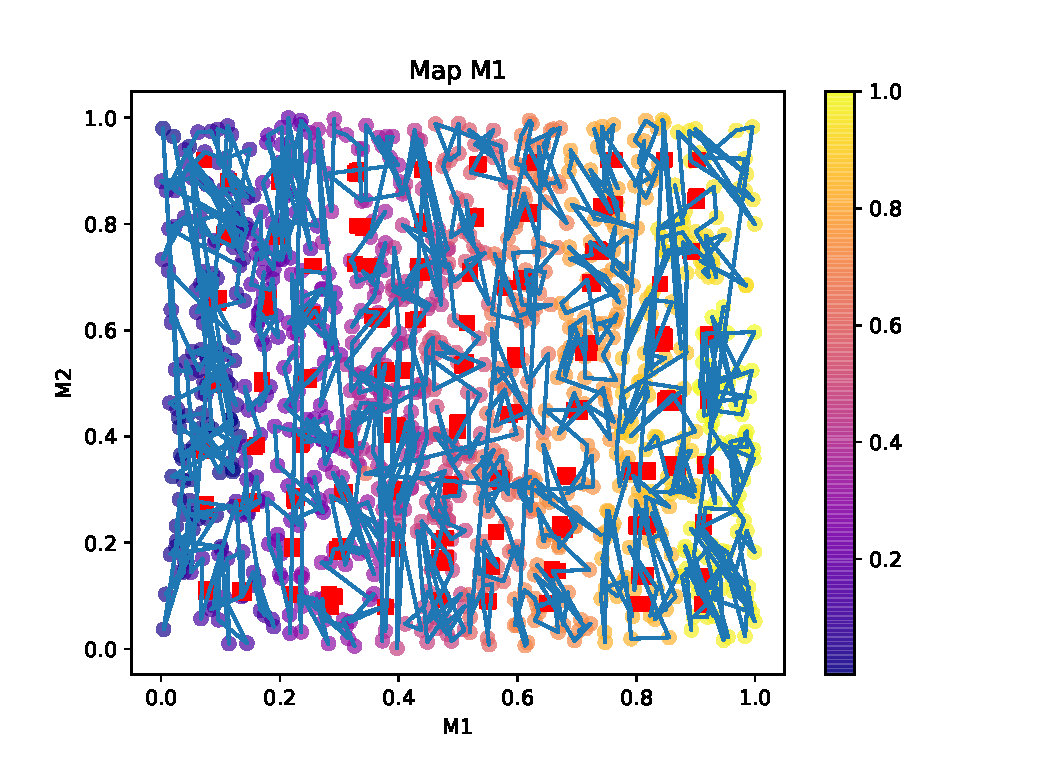
\includegraphics[width=\textwidth]{2som_square_din.pdf}
\end{minipage}
\label{fig:2som_square}
\caption{Tracé des poids de M1 et M2, dépliement des poids de M1 dans l'espace 2D et dépliement des entrées}
\end{figure}

Cette expérience montre que la disposition en vagues des cartes est un comportement lié à l'architecture et non aux données en elles même : quelles que soient les données, la carte effectuera toujours une séparation en indices primaires et secondaires. Ici, pour un X donné, on a toutes les valeurs possibles pour Y.
Cependant, les poids sont un peu différents de l'expérience avec X,Y sur un cercle : les bmus au sein d'une zone secondaire sont répartis tout le long de cette zone, alors que pour un cercle ils sont centrés dans la zone.
C'est intéressant de voir que même si seuls les poids contextuels ne nous éclairent pas trop sur le comportement des cartes, leur forme traduit quand même un aspect du modèle. 


\section{Entrées en clusters}

On considère des entrées $X$, $Y$ distribuées dans $[0,1]^2$, telles que les points sont regroupés autour de 6 centres. Autour de ces centres, les points sont tirés aléatoirement dans un cercle. On a donc des clusters de points. La distribution de $(X,Y)$ peut être considérée comme fonction des centres des clusters.  A-t-on un regroupement des points des clusters dans la carte, ou la carte se déplie t-elle sans prendre en compte les regroupement ? Nous présentons ici deux expériences, chacune prenant des entrées distribuées selon des tailles différentes de clusters autour de leurs centres, tracées en figure~\ref{fig:cluster_in}.  $U$ est ici considéré comme l'indice (entre 0 et 1) du cluster.

\begin{figure}[h!]
\begin{minipage}{0.5\textwidth}
\centering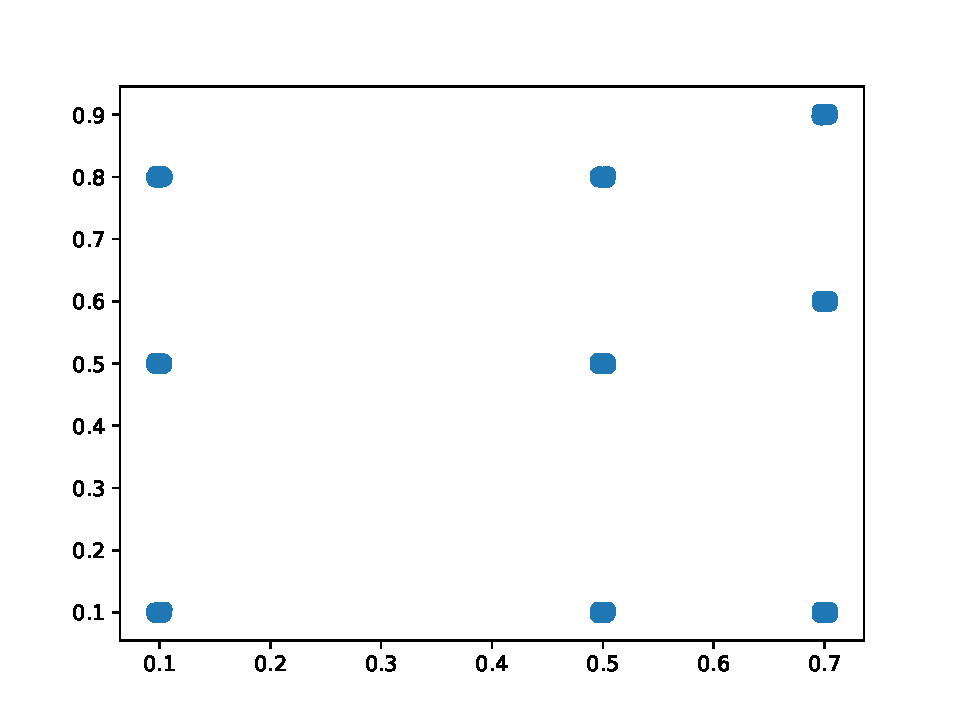
\includegraphics[width=0.7\textwidth]{2som_cluster_in}
\end{minipage}
\begin{minipage}{0.5\textwidth}
\centering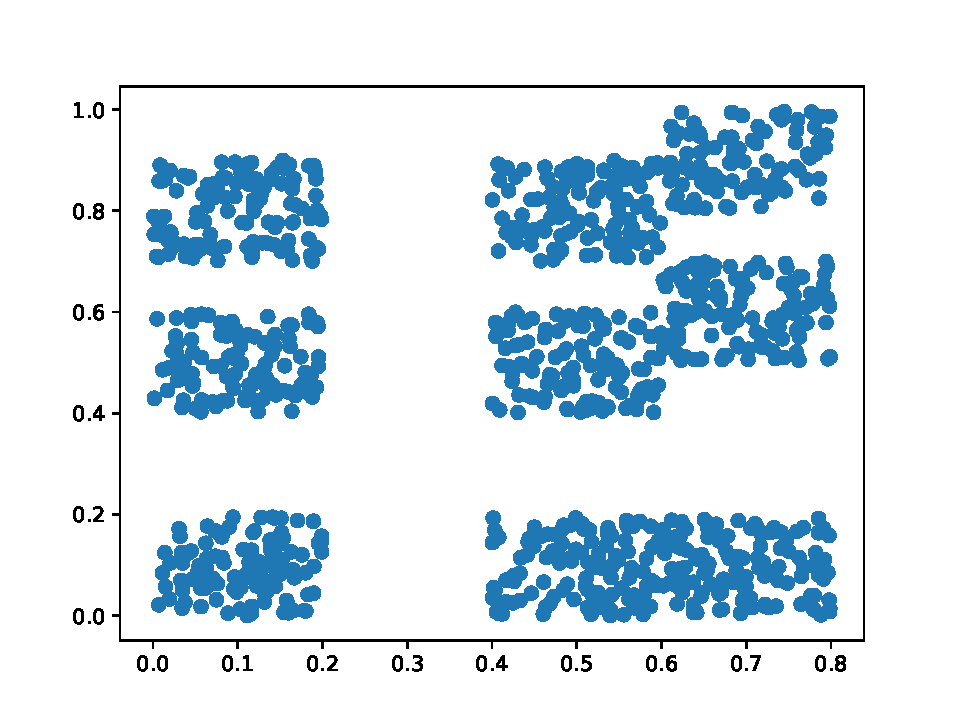
\includegraphics[width=0.7\textwidth]{2som_cluster001_in}
\end{minipage}
\caption{Entrées présentées aux cartes dans chaque expériences. A gauche, "petits" clusters, à droite, "grands" clusters}
\label{fig:cluster_in}
\end{figure}



\subsection{"petits" clusters}

\begin{figure}[h!]
\begin{minipage}{0.33\textwidth}
\centering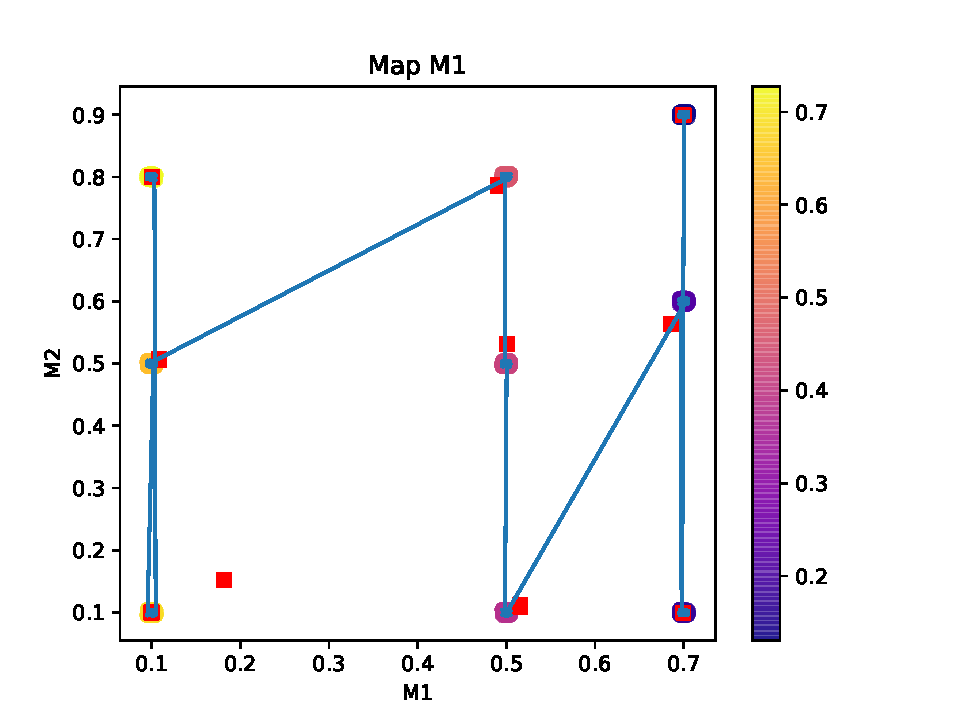
\includegraphics[width=\textwidth]{2som_cluster_din}
\end{minipage}
\begin{minipage}{0.33\textwidth}
\centering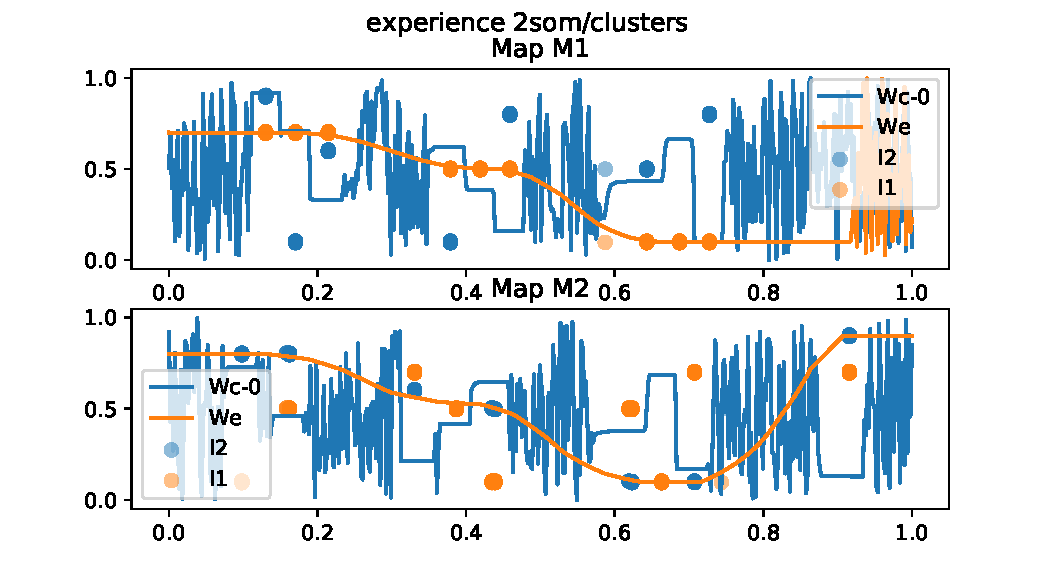
\includegraphics[width=\textwidth]{2som_cluster_w}
\end{minipage}
\begin{minipage}{0.33\textwidth}
\centering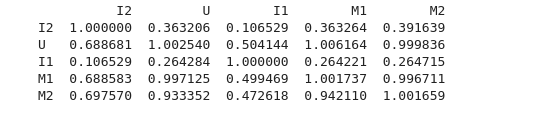
\includegraphics[width=\textwidth]{2som_clusterssmall_im.png}
\end{minipage}
\caption{Dépliement, poids et information mutuelles des cartes. }
\label{fig:cluster}
\end{figure}

La carte se déplie en suivant les clusters : un ensemble de BMU proche code pour un cluster. 

\subsection{"gros" clusters}

\begin{figure}[h!]
\begin{minipage}{0.33\textwidth}
\centering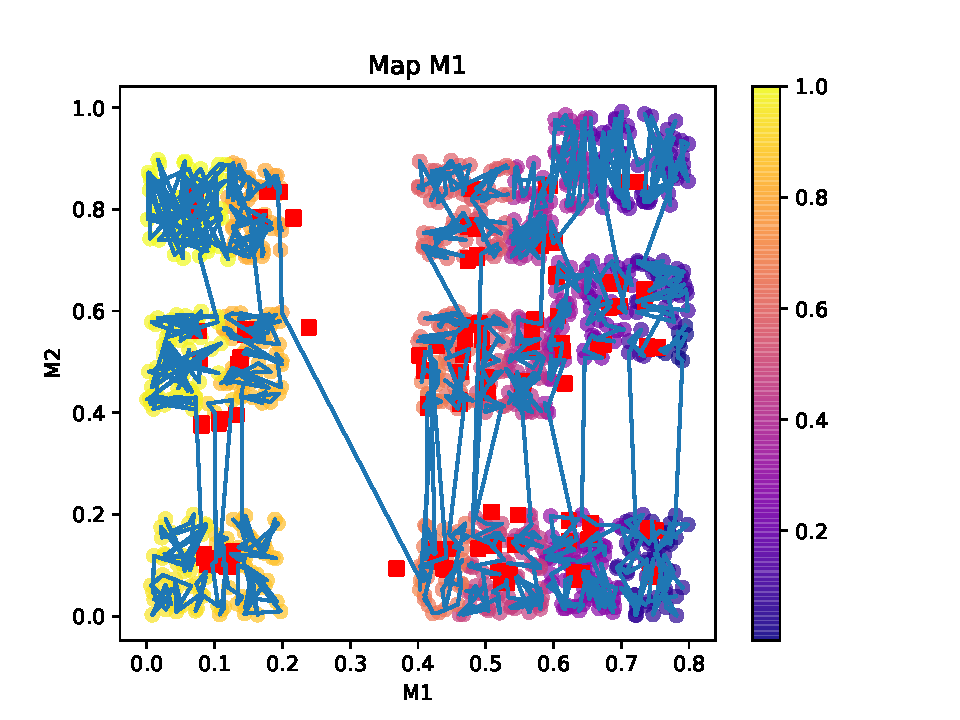
\includegraphics[width=\textwidth]{2som_cluster001_din}
\end{minipage}
\begin{minipage}{0.33\textwidth}
\centering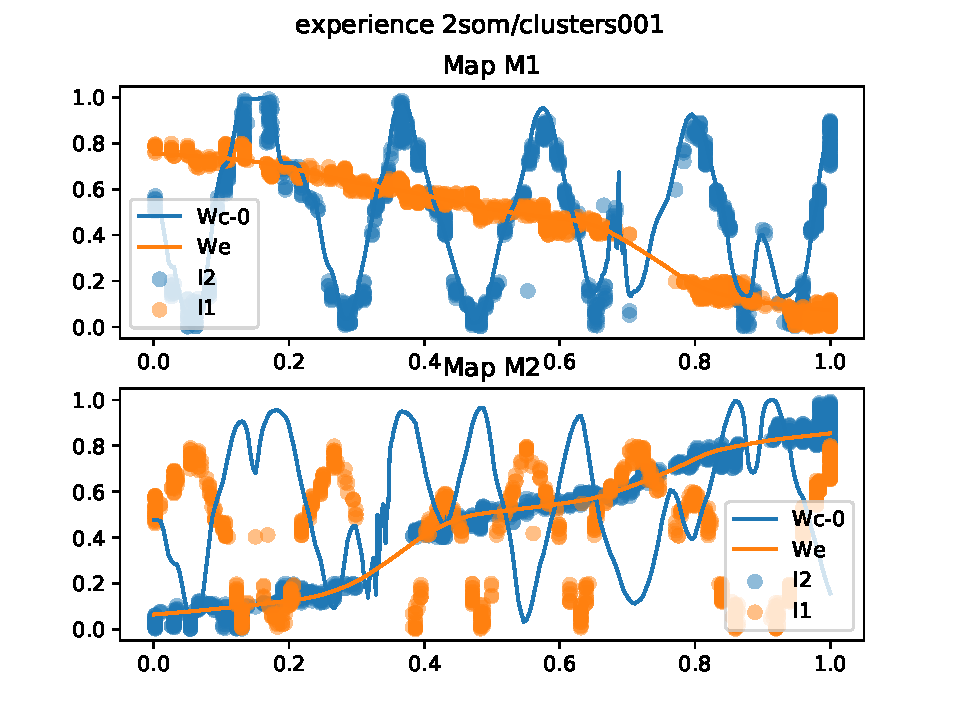
\includegraphics[width=\textwidth]{2som_cluster001_w}
\end{minipage}
\begin{minipage}{0.33\textwidth}
\end{minipage}
\caption{Dépliement, poids et information mutuelles des cartes. }
\label{fig:cluster001}
\end{figure}

La carte sépare les éléments d'un même cluster en plusieurs zones. Par contre, un ensemble de BMU code pour une partie d'un cluster, mais ne correspond  


\section{Influence de l'architecture sur des entrées}

Sur des entrées identiques, on testera différentes architectures afin d'évaluer le rôle des connexions. On utilisera toujours comme entrée dans cette section un cercle en deux ou trois dimensions. 
Comme on a vu dans les sections précédentes, l'architecture est robuste aux entrées bruitées; on utilise donc ici des entrées sans bruit. 

\subsection{Cartes intermédiaires}
mettre line 4 som, etc. 

information mutuelle dans ce cas :) comparer a la version une carte intermédiare. 
Tableau info mutuelle : faire les comparaisons. Comparaison des entrées, ce sont a peu près les mêmes donc on doit avoir les memes valeurs ok, donc ce qui nous intéresse c'est la comparaison entre M1 M2 M3 M4 etc. 

Dans cette expérience, les entrées sont $X,Y$ ou $X,Y,Z$, sur un cercle en 2D ou 3D; l'architecture est composée de 3 cartes, une prenant $X$, une prenant $X$ et une connectée aux deux autres ne prenant que les BMUs en entrée. Les cartes $X$ et $Y$ ne sont pas directement connectées. On testera l'architecture avec une et deux cartes intermédiaires pour la version 2D (figure~\ref{fig:archi_intermediaire}).
Pour la version 3D, on a une carte centrale. 

\begin{figure}[h!]
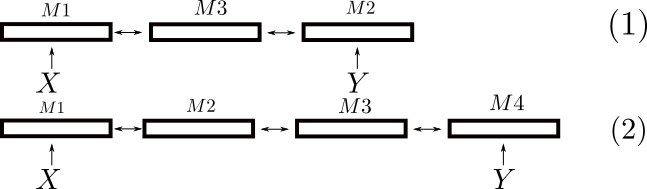
\includegraphics[width=0.7\textwidth]{archi_intermediaire.png}
\caption{Architectures avec une (1) et deux (2) cartes intermédiaires sans entrées, présentées dans cette section. }
\label{fig:archi_intermediaire}
\end{figure}

\begin{figure}[h!]
\begin{minipage}{0.5\textwidth}
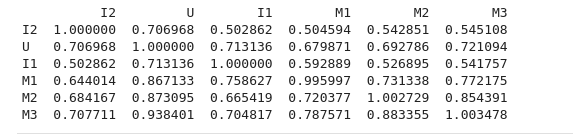
\includegraphics[width=\textwidth]{2som_star_im.png}
\end{minipage}
\begin{minipage}{0.5\textwidth}
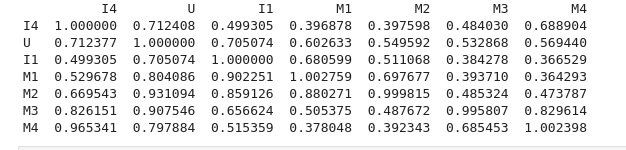
\includegraphics[width=\textwidth]{2som_line4_im.png}
\end{minipage}
\caption{coefficients d'incertitude entre les éléments des cartes, pour l'architecture (1)(gauche) et (2)(droite). Le nombre de voisins utilisés pour l'estimation est 10. L'estimation est réalisée sur 1000 échantillons. $I1$ est l'entrée de la carte $M1$ et correspond à $X$,  $I2$ ou $I4$ est l'entrée de la carte 2 ou 4 et correspond à $Y$. }
\end{figure}



\begin{figure}[h!]
\begin{minipage}{0.5\textwidth}
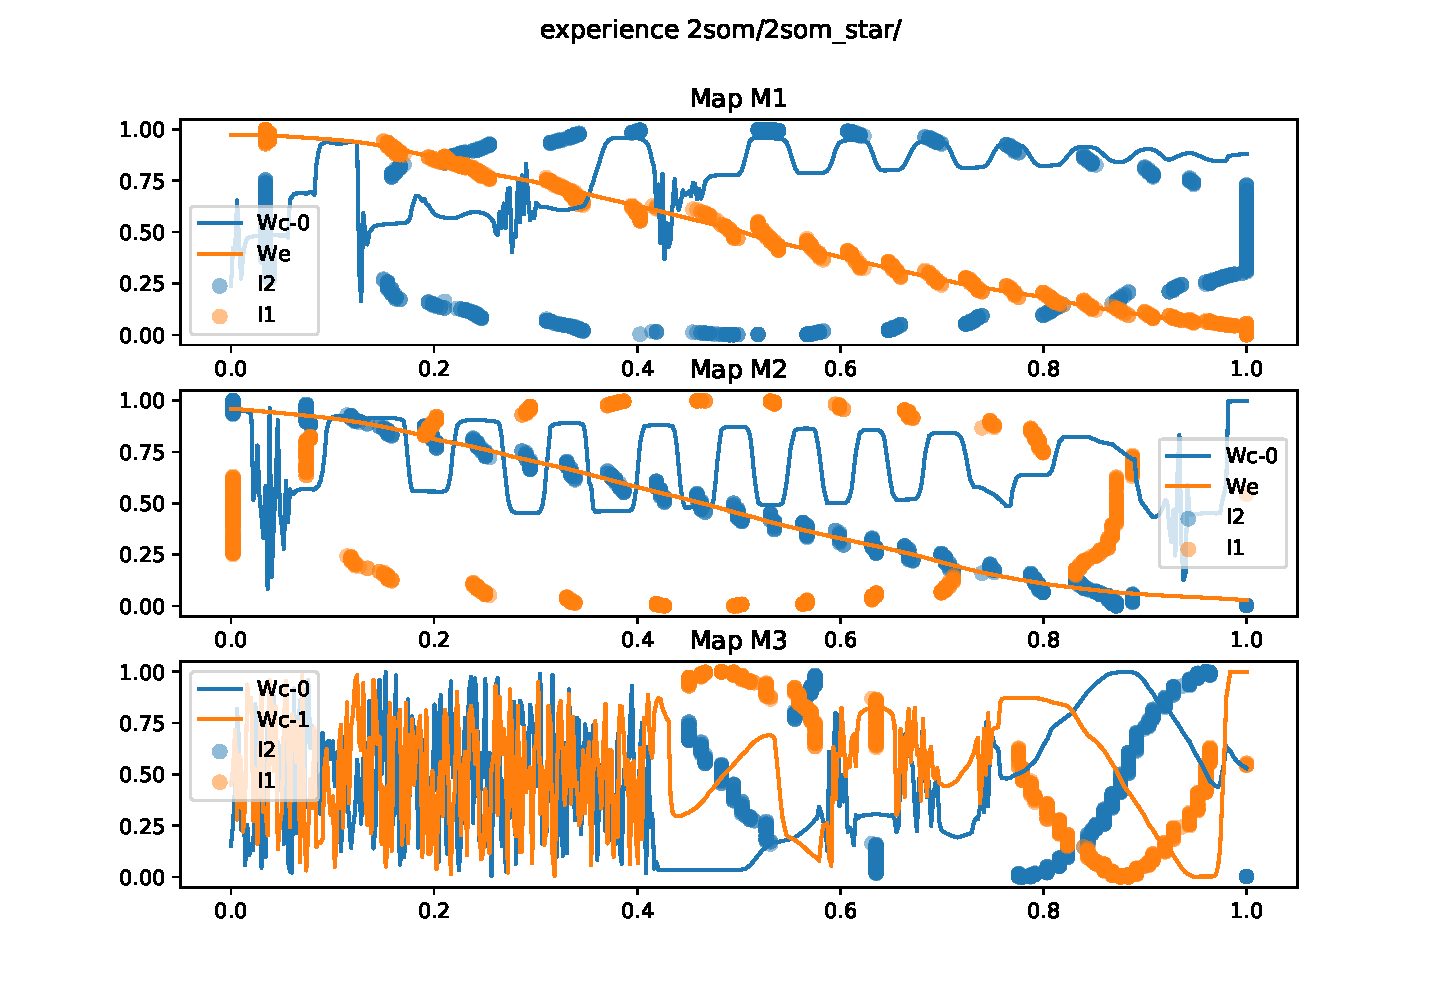
\includegraphics[width=\textwidth]{2som_star_w.pdf}
\end{minipage}
\begin{minipage}{0.5\textwidth}
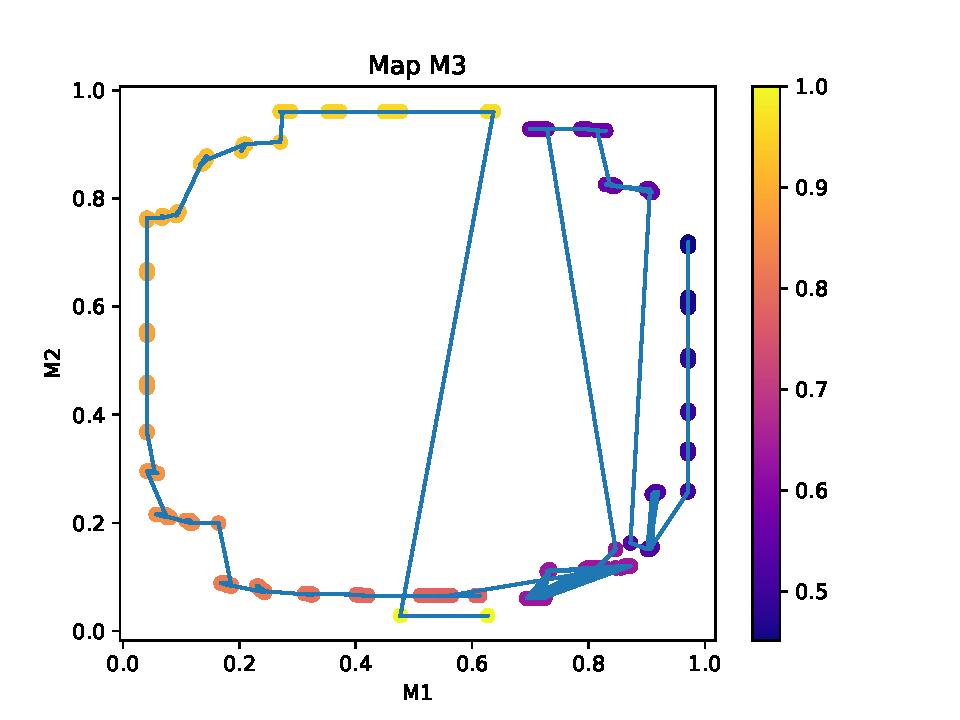
\includegraphics[width=\textwidth]{2som_star_dw3.pdf}
\end{minipage}
\caption{Poids et dépliement des deux cartes lorsqu'elles sont connectées via une carte intermédiaire (architecture (1).}
\end{figure}

% mettre ici figure avec 2 intermédiaires

\begin{figure}[h!]
\begin{minipage}{0.5\textwidth}
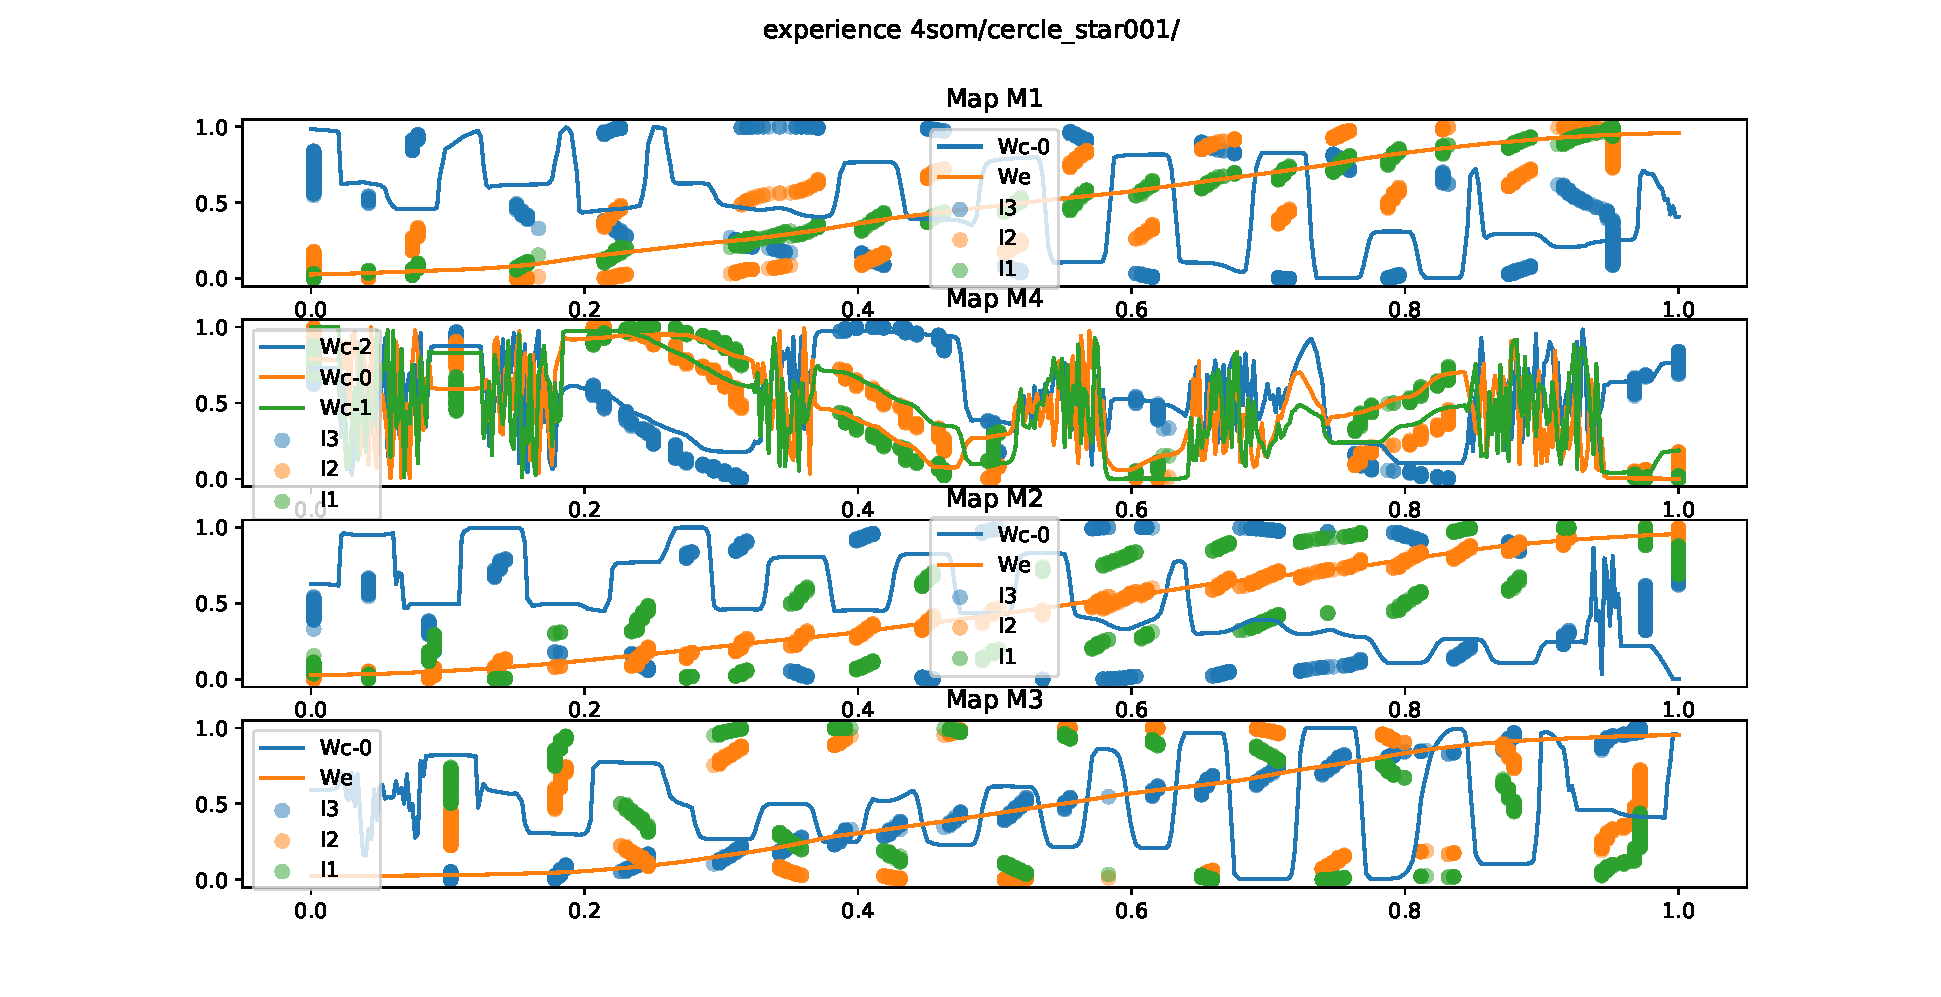
\includegraphics[width=\textwidth]{3som_star_w.pdf}
\end{minipage}
\begin{minipage}{0.5\textwidth}
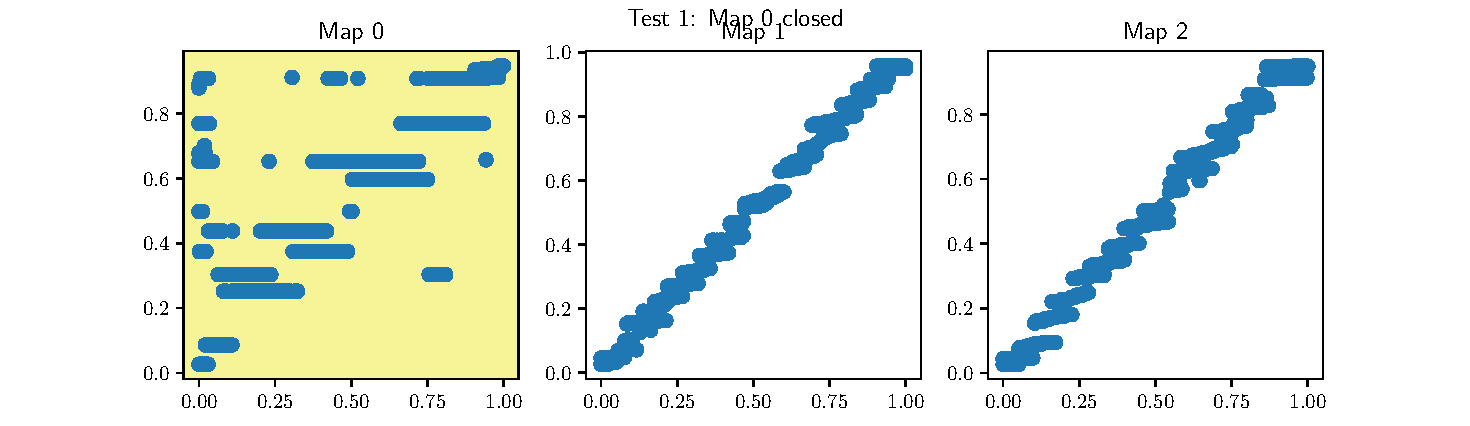
\includegraphics[width=\textwidth]{3som_star_pred.pdf}
\end{minipage}
\caption{Poids et dépliement de trois cartes connectées avec une intermédiaire.}
\label{fig:3som_star}
\end{figure}

\begin{figure}[h!]
\begin{minipage}{0.33\textwidth}
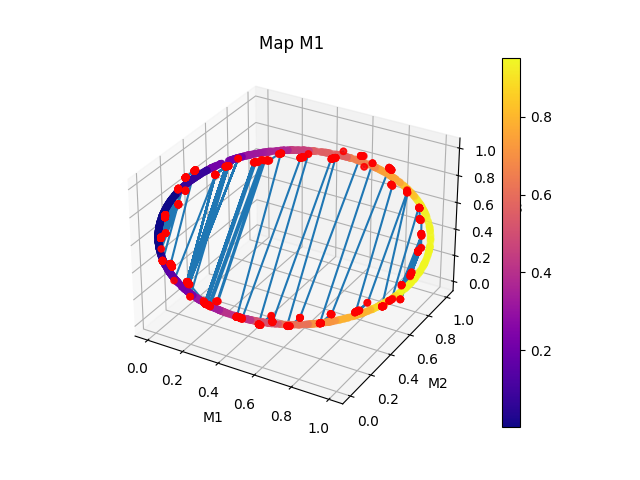
\includegraphics[width=\textwidth]{3som_star_dw1.png}
\end{minipage}
\begin{minipage}{0.33\textwidth}
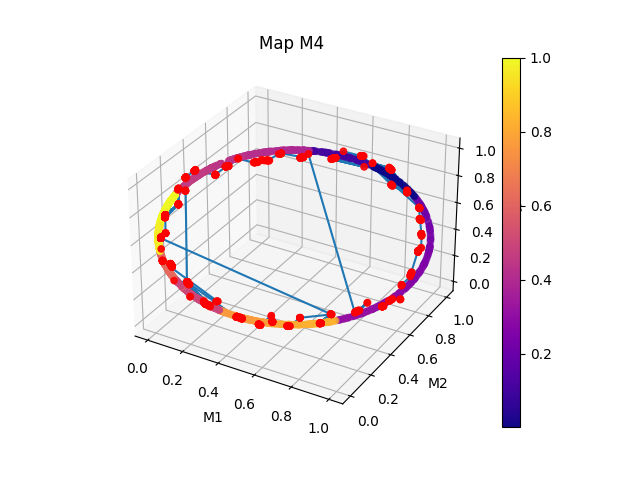
\includegraphics[width=\textwidth]{3som_star_dw4.png}
\end{minipage}
\begin{minipage}{0.33\textwidth}
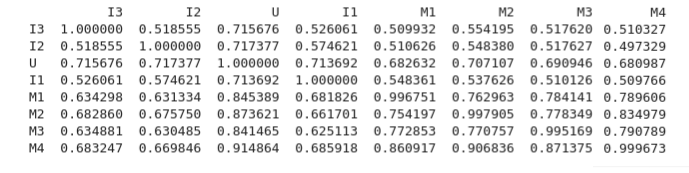
\includegraphics[width=\textwidth]{3som_star_im.png}
\end{minipage}
\label{fig:3som_star_dw}
\caption{Poids et dépliement de trois cartes connectées avec une intermédiaire et information mutuelle. Les cartes 1,2,3 recoivent des entrées, la carte 4 les connecte.}
\label{fig:3som_star}
\end{figure}

Les coefficients d'incertitudes sont ici un élément de comparaison particulièrement bon entre les cartes. Les relations entre les entrées $X$, $Y$ sont identiques, on a en effet la même distribution. 
On peut porter notre attention sur $UC(I1|M1)$ dans les deux cas : ce coefficient est plus élevé dans le cas 2.
Cela traduit une meilleure quantification vectorielle par les cartes ayant une entrée externe lorsqu'on met 2 cartes intermédiaires qu'une seule. On se rapproche en fait d'une architecture dans laquelle les cartes ne seraient pas connectées. Il semblerait donc que seules les connexions directes soient vraiment utiles. 
Par contre, on peut regarder $UC(U|M3)$ pour (1), ou $UC(U|M2)$ et $UC(U|M3)$ pour (2). 
Dans le cas (1) : le coefficient est de 0.93, vs 0.9 sur les deux cartes ayant une entrée externe, donc la différence n'est pas si significative. Les trois cartes ont une information sur le modèle.
Dans le cas (2) : le coefficient est de 0.9 sur M2 et M3, vs 0.8 sur les cartes du bout. Il semble donc que les cartes intermédiaires ont appris une représentation de la variable cachée.

On peut maintenant s'intéresser au dépliement des cartes, et à leur capacité de prédiction dans le cas en 3 dimensions. ( La prédiction n'étant en effet pas possible dans le cas de deux cartes). A trois cartes, la prédiction semble moins bonne que lorsque les trois cartes sont directement connectées. 
Si on regarde les coefficients d'incertitude, on remarque que les BMUs de la carte 4, qui connecte les trois autres, ont une info de 0.9 sur U et sur les bmus des trois autres cartes. Elle possède également un peu plus d'infos sur I1, I2, I3 que les cartes séparées. 
Donc, d'un coté la carte centrale possède les infos sur le modèle, mais d'un autre coté l'architecture effectue mal la prédiction lorsqu'une entrée manque. 

On peut donc imaginer utiliser des cartes centrales dans ce genre d'architecture pour résumer les trois autres. Ainsi, on pourra travailler sur l'info d'une seule des cartes au lieu de trois.

\subsection{Carte contextuelle de rayon 0.2}
Convergence ok, beau sinus de la carte M4 mais plus du tout de prédiction possible. Est ce que ca a un intérêt ? D'un coté, on a résumé les 3 cartes en une seule. 
Cela semble confirmer en tout cas l'implication sous-indices => prédiction. Ici pas de prédiction possible et pas de sous indices. 
 
\subsection{Et si on a la même architecture, avec une carte centrale, mais cette fois les cartes M1, M2, M3 sont également connectées ?}



\subsection{Boucle vs rétroaction à trois cartes}
On a vu avec les cartes intermédiaires que les connexions lointaines semblent jouer un role moins important dans la dynamique que les connexions directe. Ainsi, on peut regarder comment se comporte une architecture de trois cartes connectées en boucle.

\begin{figure}
\begin{minipage}{0.5\textwidth}
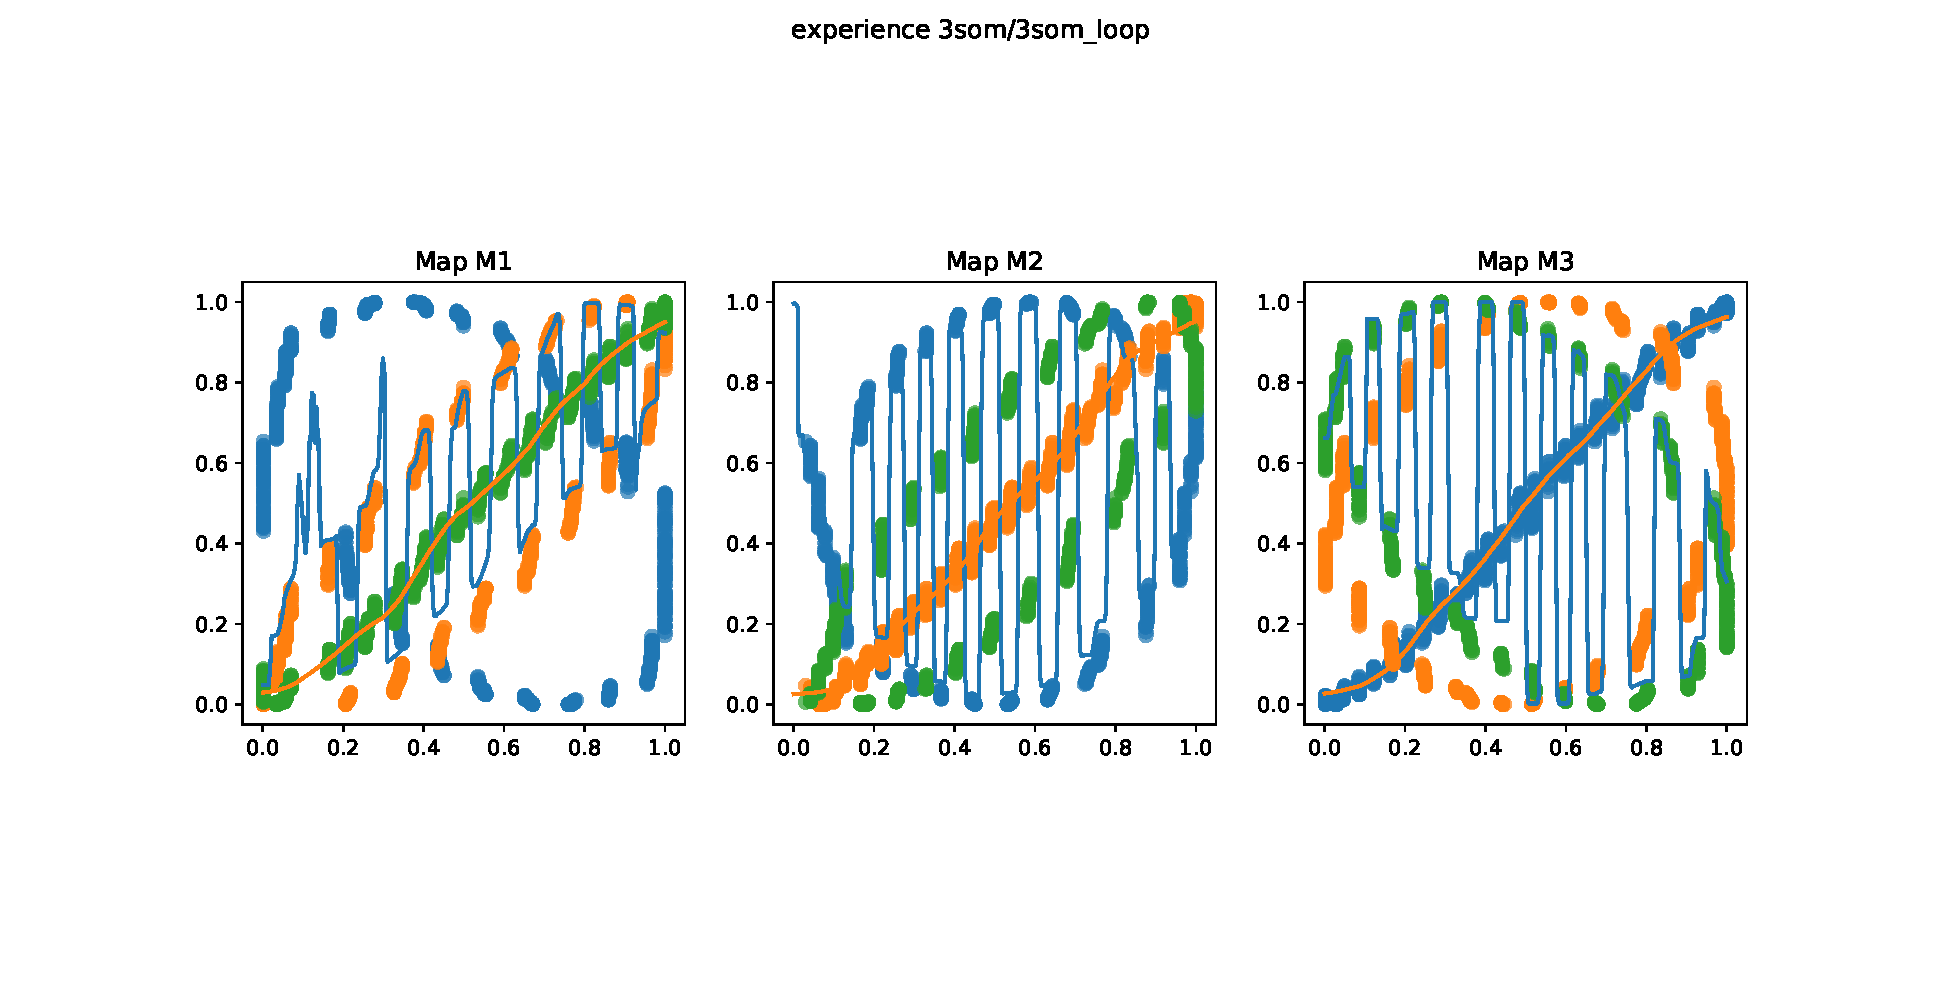
\includegraphics[width=\textwidth]{3som_loop_w.pdf}

\end{minipage}
\begin{minipage}{0.5\textwidth}
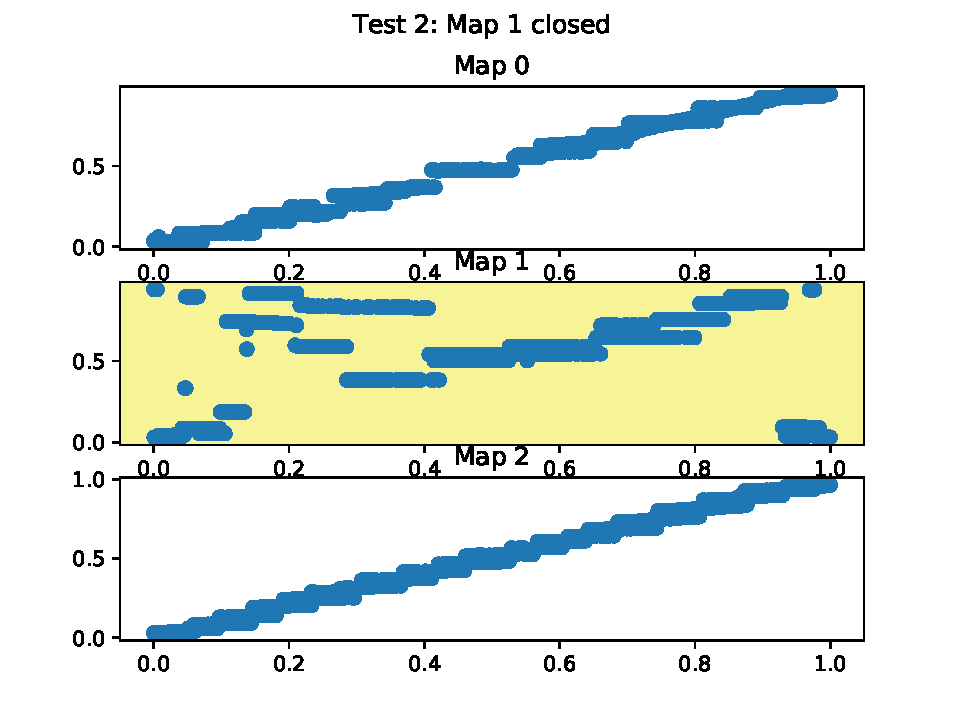
\includegraphics[width=\textwidth]{3som_loop_pred.pdf}
\end{minipage}
\caption{Poids et prédiction de trois cartes connectées en boucle (1-> 2 -> 3 -> 1). L'organisation des poids est semblable à la version en rétroaction, mais la prédiction est plus mauvaise.}
\label{fig:3som_loop}
\end{figure}

\begin{figure}
\begin{minipage}{0.45\textwidth}
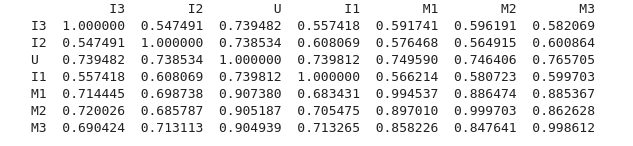
\includegraphics[width=\textwidth]{3som_cercle_im}
\caption{Coefficients d'incertitude lorque les cartes sont connectées rétroactivement, entrées sur un cercle}
\end{minipage}
\hfill
\begin{minipage}{0.45\textwidth}
\centering
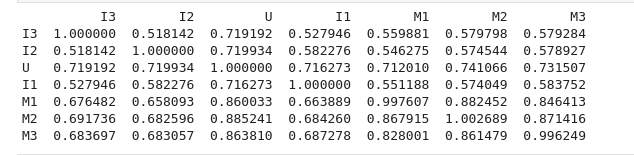
\includegraphics[width=\textwidth]{3som_loop_im.png}
\caption{Coefficient d'incertitude (colonne|ligne) lorsque les cartes sont connectées en boucle, entrées sur un cercle}
\end{minipage}
\end{figure}


\subsection{Conclusion et perspectives: influence de l'architecture}

\section{Influence des paramètres des cartes}

\subsection{rayons de voisinage}
Le rayon de voisinage des cartes, et principalement la différence entre rayons de voisinage externe et contextuel des cartes joue un gros rôle dans l'organisation. C'est cette différence de rayon de voisinage permet la séparation en indices primaires et secondaires. Lorsque les voisinages sont égaux, cette répartition ne se fait pas; mais également, les poids ne peuvent pas se stabiliser. Prendre $r_c < r_e$ permet donc une organisation stable, une séparation d'indices et une prédiction. Les paramètres sont indiqués en tableau~\ref{tab:rcre_params}.

\emph{vidéo rcre}
\begin{table}
\begin{tabular}{ l c c c }
 name & re & rc & delta\\ 
 rcre0 & 0.2 & 0.1 & 0.1\\  
 rcre1 & 0.2 & 0.07 & 0.1 \\
 rcre2 & 0.2 & 0.05 & 0.1 \\
 rcre3 & 0.2 & 0.01 & 0.1 \\
 rcre4 & 0.2 & 0.005 & 0.1
\end{tabular}
\caption{Paramètres de rayon de voisinage utilisés dans les expériences de comparaison}
\label{tab:rcre_params}
\end{table}

\subsection{Taille de la carte}

Carte grande taille, même comportement qu'avec 500 noeuds; pas d'améloriation significative.
Carte petite taille (20 noeuds) :on n'a pas assez d'unités pour faire les séparations. On a donc 8 unités qui seront bmus, mais pas de prédiction possible ou de différenciation de U par exemple. (voir figures).
Ainsi, le comportement auquel on s"intéresse, à savoir la capacité de différentiation des BMU selon le modèle, n'est plus possible. Cela pose question  :
\begin{itemize}
\item Si on veut faire des cartes 2D, on devra donc avoir des grandes cartes (100 par 100 au moins)! 
\item Même sur 500 points, on a seulement ~20 régions d'une carte qui sont utilisées, et parmi elle peu de BMU. On perd beaucoup de noeuds.
\item Si les entrées sont trop complexes (beaucoup de cartes, donc beaucoup de valeurs possible pour U), pourra t on toujours effectuer une différencitation des entrées ? 
\end{itemize}



\subsection{Combinaison des activités externes et contextuelles par moyenne ou moyenne géométrique}

\subsection{Influence de la relaxtion}

Il semble que la relaxation ne soit même plus utile lorsque 

\section{Conclusion des expériences, perspectives et limites}